\noindent{\begin{center}
\fbox{
\begin{minipage}{0.95\textwidth}
    \begin{center}
    \textbf{\textit{CELEBRAZIONI per il Santo NATALE - 2023}}
    \end{center}
\end{minipage}
}
\end{center}}

\vspace{1em}
\small

La \textbf{Novena} di Natale per giovani e adulti è da sabato 16 e fino al 23 dicembre. Da lunedì a venerdì alle ore 18.00, il sabato alle ore 18.30.

Il Triduo natalizio per i bambini sarà dal 21 al 23 alle ore 17.00.


\begin{center}
\begin{tblr}
{
    rows = {valign = m},
    column{1} = {8em, c},
    column{2} = {0.75\textwidth, l},
    hlines,
    hline{1,Z} = {1pt},
    colsep=2pt,
    rowsep=3pt
}


{Domenica 24 Dicembre} &
{
Ore \textbf{8.00 e 10.30 SS. Messe} festive. \\
Confessioni per tutto il giorno. \\
Ore \textbf{22.30}, in chiesa il Coro S. Giorgio farà alcuni canti natalizi. \\
Ore \textbf{23.00}, S. Messa nella Notte Santa.
}
\\
{Lunedì 25 Dicembre} &
{
\textbf{\textit{Natale}} \\
Ore \textbf{8.00, 9.30, 11.00. SS. Messe}. \\
Ore \textbf{16.00}. Vesperi e Adorazione eucaristica.
}
\\
{Martedì 26 Dicembre} &
{
\textbf{\textit{S. Stefano}} \\
Ore \textbf{9.00. S. Messa}.
}
\\
{Domenica 31 Dicembre} &
{
Festa della Sacra Famiglia \\
Ore \textbf{18.30. S. Messa} di fine anno col canto del \textit{Te Deum}.
}
\\
{Lunedì 1 Gennaio 2024} &
{
Festa di Maria Madre di Dio. \\
Ricorre la Giornata Mondiale della Pace. \\
Ore \textbf{8.00, 10.30. SS. Messe}. \\
Ore \textbf{16.00}. Vesperi.
}
\\
{Venerdì 5 Gennaio 2024} &
{
Ore \textbf{18.30}. Prefestiva dell’ Epifania.
}
\\
{Sabato 6 Gennaio 2024} &
{
\textbf{\textit{Epifania}} \\
Festa dei santi Magi che adorano Gesù Bambino. \\
Ore \textbf{8.00, 10.30. SS. Messe}. \\
Ore 16.00. Vesperi e conclusione col bacio a Gesù Bambino.
}
\\
{Domenica 7 Gennaio 2024} &
{
Festa del Battesimo di Gesù. \\
Ore \textbf{8.00, 10.30. SS. Messe}.
}
\end{tblr}


\vspace{1em}

\begin{minipage}{0.25\textwidth}
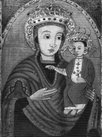
\includegraphics[width=\textwidth]{angolo.png}
\end{minipage}
\hfill
\begin{minipage}{0.72\textwidth}
Confessioni con preparazione comunitaria.

Per i giovanissimi e giovani a Maserada il giovedì 21 dicembre alle ore 20.30.

Per gli adulti a Breda martedì 19 dicembre ore 20.30 e a Candelù venerdì 22 dicembre ore 20.30.

A Maserada ci sarà un confessore straordinario oltre il parroco sabato 23 mattino e pomeriggio; la domenica 24 dalle 14.30 alle 18.00. Poi la chiesa viene chiusa fino alle ore 21.30.
\end{minipage}

\end{center}


\normalsize
